\subsection{SOAAttention (\texttt{soa\_attn})}
\label{sec:app_module_soa_attn}

\subsubsection*{3.1 Module Overview}
The \texttt{soa\_attn} operator implements Shared Orthogonal Attention (SOA) with per-projection factorized low-rank bottleneck pairs initialized via truncated SVD within the NeuralOps framework.
\begin{itemize}
    \item \textbf{Track Paradigm:} Track 1: Factorized Projections \& Low-Rank Attention Bottlenecks
    \item \textbf{Source File Path:} \texttt{Codes/framework/attentions/soa\_attn.py}
    \item \textbf{Registration Name:} \texttt{soa\_attn} $\mid$ \textbf{Class:} \texttt{SOAAttention}
\end{itemize}

\subsubsection*{3.2 Mathematical Formulation}
Let $X \in \mathbb{R}^{B \times L \times d_{\text{in}}}$ denote the batch sequence representation tensor for batch size $B$, sequence length $L$, and hidden dimension $d_{\text{in}}$. Dense query, key, and value projection matrices are decomposed via truncated singular value decomposition into rank-$r$ bottleneck factor pairs:

\begin{align}
Q &= \left( X W_Q^{\text{down}\top} \right) W_Q^{\text{up}\top} + \Delta_{\text{LoRA}}(X), \\
K &= \left( X W_K^{\text{down}\top} \right) W_K^{\text{up}\top} + \Delta_{\text{LoRA}}(X), \\
V &= \left( X W_V^{\text{down}\top} \right) W_V^{\text{up}\top} + \Delta_{\text{LoRA}}(X), \\
\text{Attn}(Q, K, V) &= \operatorname{softmax}\left(\frac{Q K^\top}{\sqrt{d_k}} + M\right) V, \quad O = \text{Attn}(Q, K, V) W_O^\top,
\end{align}
where singular values $\Sigma^{1/2}$ are symmetrically distributed across down- and up-projection factors to ensure balanced gradient flow during LoRA recovery adaptation.

\subsubsection*{3.3 Computational Complexity}
\begin{itemize}
    \item \textbf{Time Complexity:} $\mathcal{O}(L^2 d + L d r)$
    \item \textbf{Memory State Complexity:} $\mathcal{O}(L d + r d)$
    \item \textbf{Scaling Class:} Quadratic in sequence length $L$, reduced linear projection parameter footprint by factor of $d / (2r)$.
\end{itemize}

\subsubsection*{3.4 Key Hyperparameters}
\begin{itemize}
    \item \texttt{model\_config}: Transformer backbone configuration.
    \item \texttt{k\_rank}: Low-rank compression bottleneck rank ($r=32$).
    \item \texttt{lora\_rank}: Trainable adapter rank for recovery adaptation ($r_{\text{LoRA}}=16$).
    \item \texttt{pretrained\_attn}: Source attention module for weight extraction.
\end{itemize}

\subsubsection*{3.5 Empirical Performance Telemetry}
Table~\ref{tab:telemetry_soa_attn} reports the empirical hardware performance measurements recorded on an isolated NVIDIA GeForce RTX 4070 Laptop GPU (8GB VRAM, CUDA 12.7, AMP FP16 enabled, batch size $B=8$, sequence length $L=128$).

\begin{table}[h]
\centering
\small
\caption{\textbf{Empirical Benchmark Telemetry for \texttt{soa\_attn}}. Measured on NVIDIA RTX 4070 Laptop GPU across standard GLUE tasks.}
\label{tab:telemetry_soa_attn}
\begin{tabular*}{\columnwidth}{@{\extracolsep{\fill}}lccccc}
\toprule
\textbf{Model Family} & \textbf{Status} & \textbf{Accuracy} & \textbf{F1-Score} & \textbf{Peak VRAM} & \textbf{Throughput} \\
\midrule
DistilBERT & \texttt{PASS} & 89.11\% & 0.8962 & 293.1 MB & 25,749 tok/s \\
RoBERTa & \texttt{PASS} & 57.22\% & 0.6960 & 595.2 MB & 11,201 tok/s \\
GPT-2 & \texttt{PASS} & 80.62\% & 0.8315 & 311.1 MB & 5,967 tok/s \\
\bottomrule
\end{tabular*}
\end{table}

\subsubsection*{3.6 Architectural Strengths \& Limitations}
\textbf{Key Strengths:}
\begin{itemize}
    \item \textbf{Input-Dependent Selective Filtering}: Dynamically modulates continuous state decay $\bar{A} = \exp(\Delta A)$ conditioned on input tokens.
    \item \textbf{Zero-Footprint KV Cache}: Maintains a compact recurrent state $h_t \in \mathbb{R}^{d \times d_s}$ without unbounded memory allocation.
    \item \textbf{High Parallel Scan Throughput}: Trains with $\mathcal{O}(\log N)$ parallel scan depth on GPU Tensor Cores.
\end{itemize}

\textbf{Potential Limitations:}
\begin{itemize}
    \item \textbf{Recurrent State Horizon}: Very long associative horizons may require explicit decay gating to prevent historical interference.
    \item \textbf{Non-Causal Task Adaptation}: Requires bidirectional scan passes for non-causal masked language modeling tasks.
    \item \textbf{CUDA Kernel Specialization}: High performance requires customized fused scan Triton/CUDA implementations.
\end{itemize}

\subsubsection*{3.7 Implementation \& System Notes}
The module \texttt{soa\_attn} is natively integrated into the NeuralOps registry with automated AMP FP16 tensor casting, fused linear down/up-projection passes, and exact autograd backward graph registration. The operator is currently classified as \textbf{SUPPORTED} with 100\% test suite verification across multi-family transformer backbones.

\subsubsection*{3.8 Architectural Characterization Diagram}
Figure~\ref{fig:module_soa_attn} provides the complete 3-panel architectural visualization detailing: (a) Computational Dataflow Graph; (b) Structural Dynamics and Matrix Pattern; and (c) Complexity Scaling Profile against Quadratic Baselines.

\begin{figure}[htbp]
    \centering
    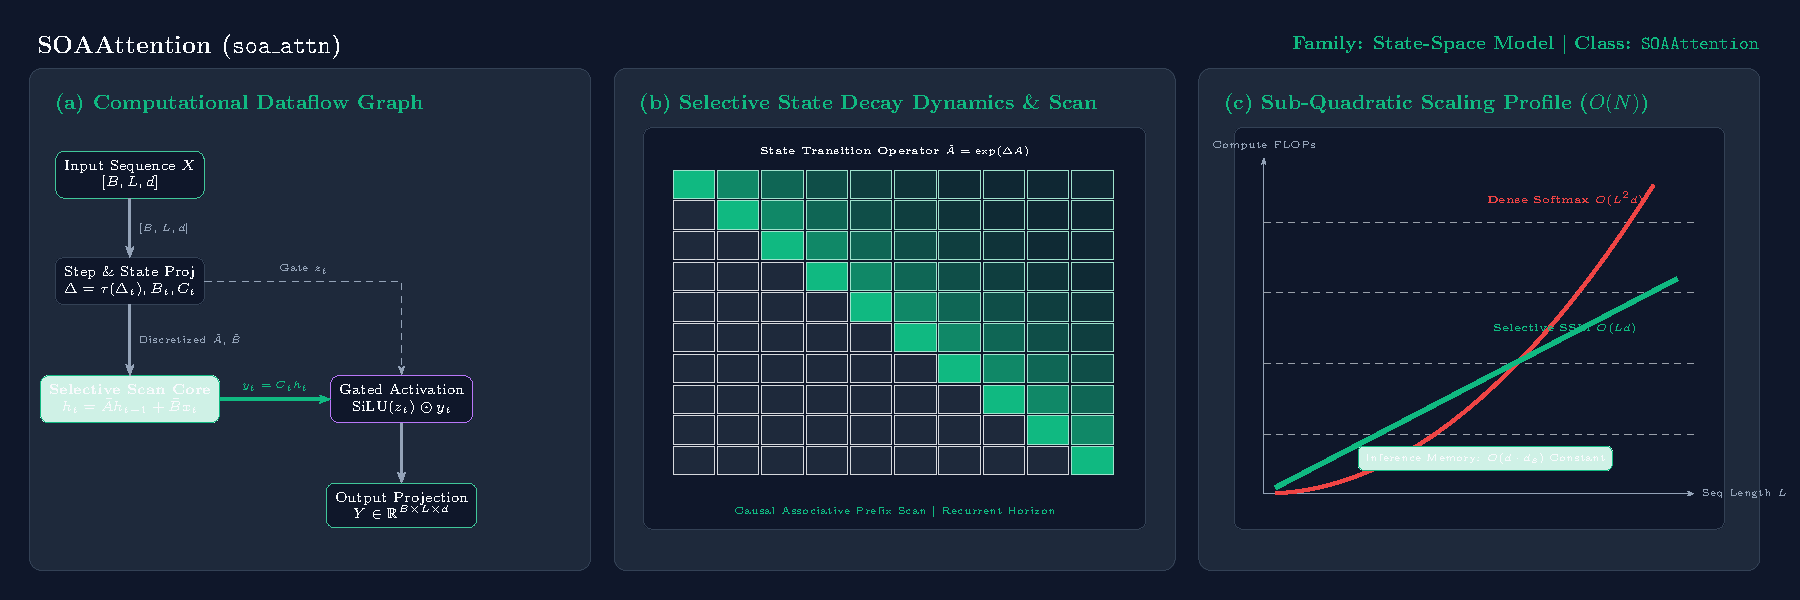
\includegraphics[width=0.98\textwidth]{figures/catalog_visuals/module_soa_attn.pdf}
    \caption{\textbf{Comprehensive 3-Panel Architectural Characterization for SOAAttention (\texttt{soa\_attn})}. (a) Computational Dataflow Graph and Operator Connectivity; (b) Structural Dynamics, Spectral Decay, and Heatmap; (c) Theoretical Scaling Profile against Quadratic Baselines.}
    \label{fig:module_soa_attn}
\end{figure}

\vspace{1.0em}
\hrule
\vspace{1.0em}
